% vim: expandtab softtabstop=2 shiftwidth=2 foldmethod=marker spell

\section{Tagging Songs}
Songs are able to be tagged, and then sorted by those tags. This is especially useful when streamers form collaborations, and they want to share a single songlist. By tagging all of the newly added songs for the collaboration, you are able to mass edit them, mostly to make them active or inactive, allowing these songs to be hidden from the users when the streamers are performing separately.

In the table below, you can see what an example of how the tags have been implemented in the current backup file. In the header row, the columns \mbox{\lstinline{TAG=NAME\_OF\_TAG}} have been added and a 0 or 1 are used in the following rows to indicate if the song has that tag. Tags are not able to be imported, so these columns must be deleted before importing the songs.


\begin{table}[h!]
\pgfplotstabletypeset[col sep=comma,
  string type,
  columns={title,artist,TAG=Love},
  every head row/.style={before row=\hline,after row=\hline},
  every last row/.style={after row=\hline},
  every even row/.style={before row=\rowcolor[gray]{0.9}},
  every first column/.style={column type/.add={|}{}},
  every column/.style={column type/.add={}{|}},
  ]{src/songlist_import/example.csv}
\caption{Songlist Tag Example CSV}
\label{tag_example.csv}
\end{table}

\clearpage
On The Tags Page, you can see an overview of the current tags. Currently, the values should always be set to \lstinline{Yes}. In the future, it may be possible to easily make all of the songs with a tag active/inactive, but currently the tags page is mostly useless.

\begin{figure}[ht!]
  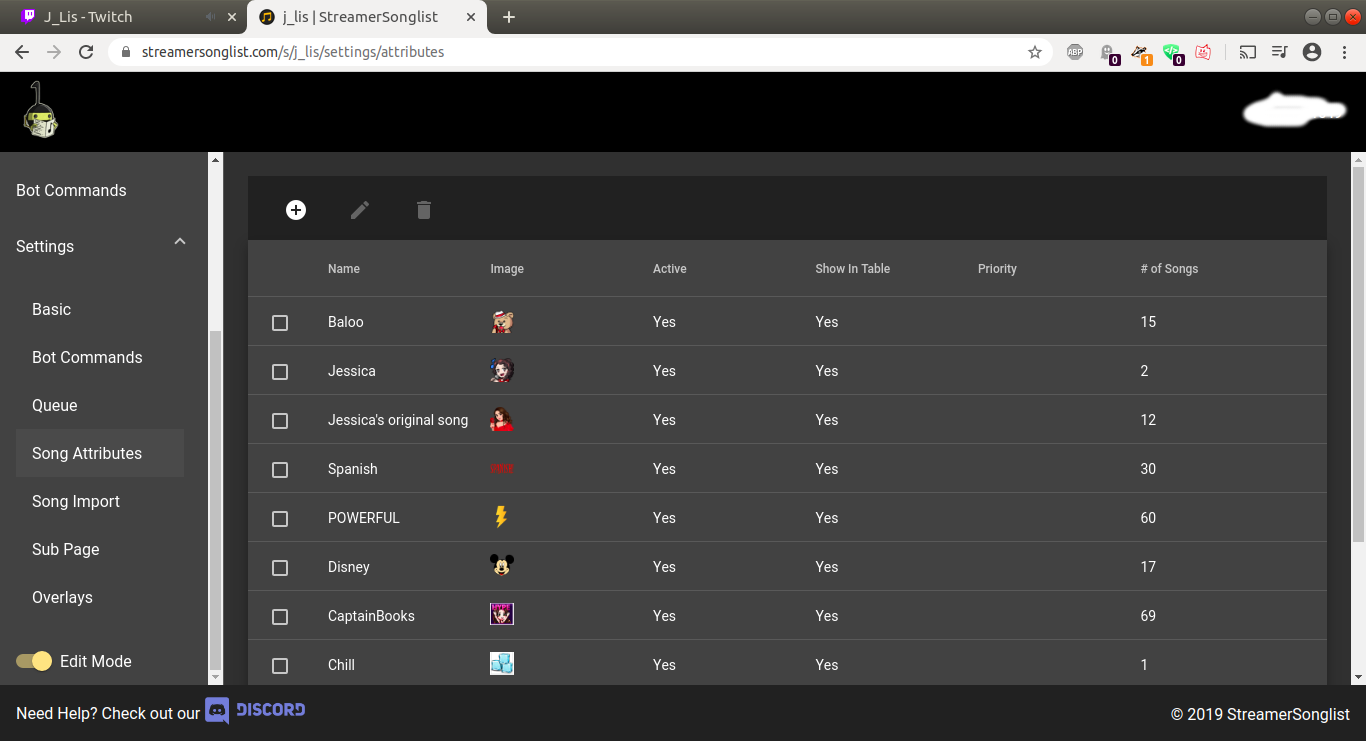
\includegraphics[width=\linewidth]{src/tags/tags.png}
  \caption{The Tags page}
  \label{tags_page}
\end{figure}
